\documentclass{article}

\usepackage{url}
\usepackage{color}
    \definecolor{darkblue}{RGB}{6,69,173}
\usepackage{hyperref}
    \hypersetup{
        colorlinks=true,
        linkcolor=darkblue,
        urlcolor=darkblue
    }

\usepackage{graphicx}

\begin{document}

\title{%
    Git Gud \\
    \large Or How To Never Lose Your Work Again}
\author{Cat Flynn}

\maketitle
\pagenumbering{gobble}
\newpage
\tableofcontents
\newpage
\pagenumbering{arabic}

\section{Introduction}
I'm sure all of us have lost a project or two thanks to unexpected failures, like a UE update corrupting your project beyond recognition or your expensive motherboard suddenly crapping out after only a year and a half. We didn't back it up because we're \textit{lazy}, and \textit{maybe I'll do it later}. It's easy to make excuses, and to say what you should have done in hindsight, but the truth is that \textit{there is a better way}.

\section{What's Git?}
Git is a tool used by developers primarily as insurance, and secondarily as a system for collaboration. It tracks incremental updates to a project and distributes them between multiple locations, such as servers and other developers' machines. Imagine setting checkpoints in your project every time you fix a bug, or implement a feature. You can track what work you did and when you did it, with the bonus of having your precious work safely out of harm's way if your PC explodes!

\section{Alright, I'm sold. How do I use Git?}
Start by downloading Git from \href{https://git-scm.com/}{git-scm.com}, and installing it. The default options should be totally fine, so go ahead and click right through. Once you're done instaling, you'll be greeted by a \textit{hacker} looking terminal (\ref{fig:terminal}). Don't be scared of it, there are only a few commands you'll need to know to be able to use Git effectively. The command line is fun, trust me!

\begin{figure}
    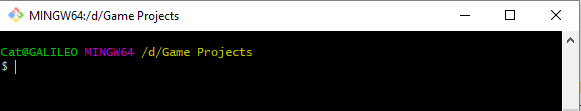
\includegraphics[width=\linewidth]{images/terminal.png}
    \caption{\textit{*hacker voice*} I'm in}
    \label{fig:terminal}
\end{figure}

\paragraph{}
The main thing to note the yellow text, which is the location in your filesystem that Git is currently running in. You can use the command \texttt{ls} to list the files and folders in this directory, and \texttt{cd} to navigate in and out of these folders. The command \texttt{cd ..} will take you to the current folder's parent; for example, running \texttt{cd ..} in the prompt shown in \ref{fig:terminal} would take me to the \texttt{/d/} folder. Lastly, the \texttt{clear} command will clear the screen, giving you a blank terminal to work with.

\paragraph{}
Before we get into using Git, let us take a moment to properly configure it. We need to give it an email and a name, so that it can attach this information to any work we do. This is required, and Git won't work without it. Run the \texttt{git config} commands as shown in \ref{fig:config} to accomplish this.

\begin{figure}
    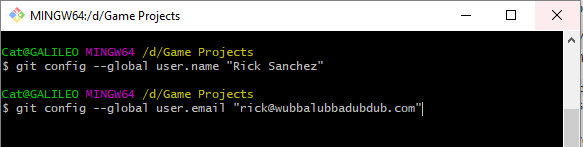
\includegraphics[width=\linewidth]{images/config.png}
    \caption{Git configuration.}
    \label{fig:config}
\end{figure}

\paragraph{}
Great! Now it's time to set up a project. This guide is primarily aimed at users of the Unity game engine on Windows, but the steps outlined will work for any project, on any system. Go ahead and create your project as normal (or you can use an existing project) and get it open in File Explorer.

\paragraph{}
Before we continue, make sure you've enabled file extenations and hidden folders in File Explorer. These options are accessed from the View tab. Right click anywhere in this folder and select `Git Bash here'. A terminal like the one we opened earlier should appear, and you'll notice the yellow path matches the filepath of your project.

\begin{figure}
    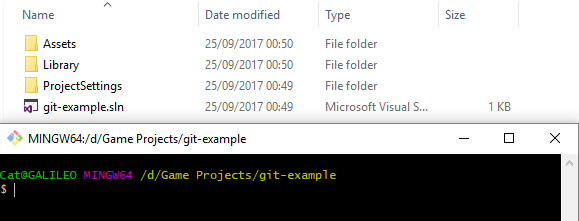
\includegraphics[width=\linewidth]{images/pre-init.png}
    \caption{Opening Git Bash in a particular folder.}
    \label{fig:pre-init}
\end{figure}

\paragraph{}
Now run the command \texttt{git init}. This command creates a `repository' in this folder. Git stores the repository state in this folder. The repository is how Git is able to share your project with others. It builds a history of changes, tracking who changed what in which files and when they did it. 

\begin{figure}
    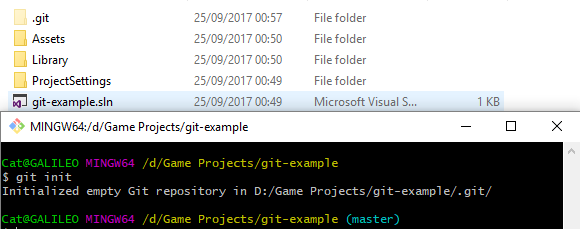
\includegraphics[width=\linewidth]{images/post-init.png}
    \caption{A project with an initialised Git repository.}
    \label{fig:post-init}
\end{figure}

\paragraph{}
You'll immediately notice a couple of things. First, there's now a faded-looking \texttt{.git} folder (\ref{fig:post-init}) sitting alongside your project. This is where Git stores whatever it needs to worry about, you shouldn't ever have to go looking in there. However, you should note that this folder needs to stay in the project root for Git to work properly. Second, there is now a blue \texttt{(master)} label after the filepath in Git's command prompt. This is the name of the current \textit{branch} you're on. Since Git stores projects as a tree, it must have at least one branch. The \texttt{master} branch is created be default in a Git repository. You can rename, add and remove branches from a repository at your leisure, but that isn't in the scope of this guide. One branch is plenty for now! As a handy tip, if there is no branch in the command prompt then that means there's no repository present either.

\paragraph{}
Now, let's make our first commit! Start out by running the command \texttt{git status} to view the current state of the repository. As seen in figure \ref{fig:status} this command outputs the folders in our project, highlighted in red because they're currently not being tracked by Git.

\begin{figure}
    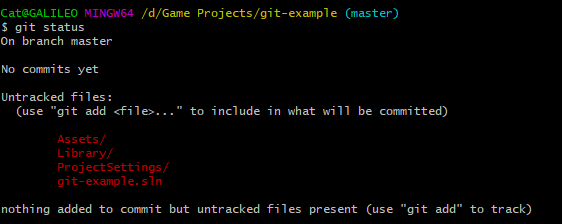
\includegraphics[width=\linewidth]{images/status.png}
    \caption{Output of \texttt{git status}.}
    \label{fig:status}
\end{figure}

\section{So what about working in a team?}
\section{Keeping it clean}
\section{Before you disappear!}

\end{document}
